\documentclass[table, czech]{beamer}
\usepackage[utf8]{inputenc}
\usepackage[czech]{babel}
\usepackage{array}
\usepackage{amsthm}
\usepackage{graphicx}
\usepackage{listings}
\usepackage{subfig}
\usepackage{float}
\usepackage{multirow}
\usepackage{booktabs}
\usepackage{color}
\usepackage{alltt}
\usepackage{algorithm}
\usepackage{algpseudocode}

% additional commands
\newcommand{\setHelper}[1]{\left\lbrace #1 \right\rbrace}

% beamer settings
\usetheme{CambridgeUK}
\setbeamertemplate{footline}[frame number]
\setbeamercolor{block title}{fg=cambridgedarkblue,bg=white}
\setbeamercolor{block body}{fg=black,bg=white}
\newtranslation[to=Czech]{Definition}{Definice}

\floatname{algorithm}{Algoritmus}
\renewcommand{\algorithmiccomment}[1]{// #1}

% title page
\title{Paralelizace algoritmu pro hledání\\maximálních nezávislých množin}
\author{Milan Munzar, Jakub Sochor}
\institute[FIT]{Fakulta informačních technologií VUT v Brně}

\begin{document}

\frame[plain] { \titlepage }
\frame
{
    \frametitle{Maximální nezávislé množiny}
\begin{definition} 
Mějme neorientovaný graf G(V, E). Podmnožinu $S \subseteq V$ nazveme maximální nezávislou množinou právě tehdy, když platí:

\begin{equation*}
\forall v_1, v_2 \in S: (v_1, v_2) \notin E\ \wedge\ \forall v' \in V \setminus S: Adj(v') \cap S \neq \emptyset
\end{equation*}
\end{definition}
\begin{itemize}
    \item $NP$-úplný problém
\end{itemize}

}

\frame
{
    \frametitle{Algoritmus pro hledání maximálních nezávislých množin}
    \begin{itemize}
        \item Využívá backtracking
        \item Používá vzájemně disjunktní množiny uzlů $N$, $S$, $R$
        \begin{itemize}
            \item $N$ -- zatím nevyzkoušeno
            \item $S$ -- již vyzkoušeno přidání
            \item $R$ -- nezávislá množina
        \end{itemize}
        \item Množiny $N$, $S$, $R$ udržovány v matici
        \item Časová složitost $O(2^{\frac{n}{3}})$
        \item Prostorová složitost $O(\alpha(G) \cdot n)$
    \end{itemize}
}

\frame
{
    \frametitle{Algoritmus pro hledání maximálních nezávislých množin}
    \begin{enumerate}
        \item Postupně se zanořuje a rozšiřuje množinu $R$
        \item Testuje, jestli množina $R$ je maximální nezávislá množina
        \item Testuje, jestli je $R$ možné zvětšit na novou maximální nezávislou množinu 
        \item Případně se navrací a upravuje stavy množin $N$, $S$, $R$
    \end{enumerate}  
}

\frame
{
    \frametitle{Paralelizace algoritmu}
\begin{algorithmic}
\Function{parIndSets}{Graph $G$}
\State $independent\_sets \leftarrow \emptyset$
\State $N_0 \leftarrow V$
\State $R_0, S_0 \leftarrow \emptyset$
\For{$v \in V$}  
    \State $seqIndSets(G, v, N_0, R_0, S_0, independent\_sets)$ in parallel
    \State $N_0 \leftarrow N_0 \setminus \setHelper{v}$
    \State $S_0 \leftarrow S_0 \cup \setHelper{v}$
    \If{$\exists y \in S_k :  Adj(y) \cap N_k = \emptyset$}
        \State \textbf{break}
    \EndIf
\EndFor
\State \Return $independent\_sets$
\EndFunction
\end{algorithmic}

}

\frame
{
    \frametitle{Použité prostředky}
    \begin{itemize}
        \item C++
        \item Boost
        \item C++11: \texttt{thread}, \texttt{mutex}, \texttt{high\_resolution\_clock}
    \end{itemize}

}


\frame
{
    \frametitle{Porovnávní se sekvenčním algoritmem}
    \begin{itemize}
        \item 4 fyzická jádra 3\,GHz, 4\,GB RAM
        \item Zrychlení kolem 3,5
        \item Klesá s počtem maximálních nezávislých množin
    \end{itemize}

    \begin{center}
        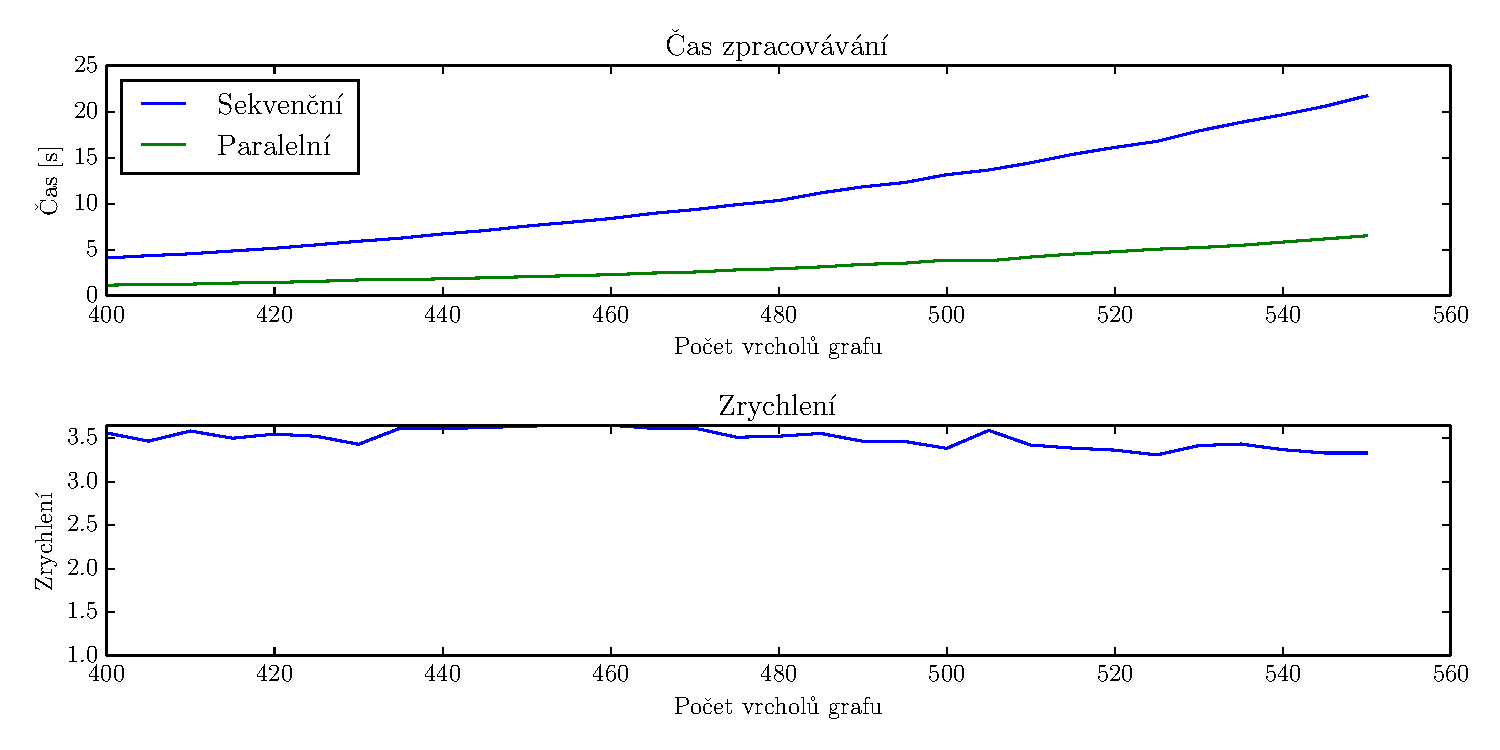
\includegraphics[scale=0.43]{./images/7.pdf}
    \end{center}    
}


\frame
{
\frametitle{Reference}
\begin{thebibliography}{99}

\bibitem{demel} 
    DEMEL, Jiří. \emph{Grafy a~jejich aplikace}. Vyd. 1. Praha: Academia, 2002, 257 s. ISBN 80-200-0990-6.

\bibitem{tarjan}
  TARJAN, Robert Endre, TROJANOWSKI Anthony E.
  \emph{Finding a~maximum independent set.}
  SIAM Journal on Computing 6.3 (1977): 537-546.

\end{thebibliography}
}

\end{document} 

